\documentclass[a4paper,10pt]{article}
% UTF8 Charset für Umlaute/Sonderzeichen
\usepackage[utf8]{inputenc}
% Deutsche Namen und Datumsformat
\usepackage[ngerman]{babel}
%Quellenangaben
\usepackage{hyperref}
%Fancy Mathesymbole
\usepackage{amssymb}
\usepackage{dsfont}
%Aufzählung
\usepackage{paralist}
%Pfeile
\usepackage{amsmath}
\makeatletter
\newcommand{\xRightarrow}[2][]{\ext@arrow 0359\Rightarrowfill@{#1}{#2}}
\makeatother
%Krams
\usepackage{amsmath}
\usepackage{amsthm}
%Gewitter
\usepackage{ stmaryrd }
% Algorithmen Pseudocode
\usepackage[]{algorithm2e}
% Bilder
\usepackage{graphics}
\usepackage{wrapfig}
%GeoGebra
\usepackage{tikz}
\usepackage{tkz-euclide}
\usetikzlibrary{arrows,automata,positioning}

\tikzset{
	state/.style={
		circle,
		draw=black, very thick,
		minimum height=2em,
		inner sep=2pt,
		text centered,
	},
}



\newcommand{\bigo}{\ensuremath{\mathcal{O}}}
\newcommand{\BT}{\ensuremath{\Theta}}
\newcommand{\N}{\ensuremath{\mathbb{N}}}
\newcommand{\Set}{\ensuremath{\mathcal{S}}}
\newcommand{\PMenge}{\ensuremath{\mathcal{P}}}
\newcommand{\Point}[2]{\ensuremath{\begin{pmatrix}#1\\#2\end{pmatrix}}}
\newcommand{\xp}{\ensuremath{x_{post}}}
\newcommand{\yp}{\ensuremath{y_{post}}}
\newcommand{\zp}{\ensuremath{z_{post}}}


% Hier die Nummer des Blatts, Autoren und Name des Betreuers angeben.
\newcommand{\blatt}{9}
\newcommand{\autor}{Edenfeld, Lemke, Moser, Schinke}
\newcommand{\betreuer}{Carina Pilch}
\usepackage{../abgabe}

\begin{document}
	% Seitenkopf mit Informationen
	\kopf
	
	\aufgabe 1

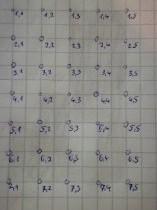
\includegraphics[width=0.33\textwidth]{1a.jpeg}


\subsection*{Aufgabenteil a:}
$v=\{(2,3),(2,4),(3,3),(3,4),(4,3),(4,4),(5,2),(5,3),(5,4),(6,1),(6,2),(6,4),(7,1),(7,2),(7,3),(7,4)\}$

\subsection*{Aufgabenteil b:}

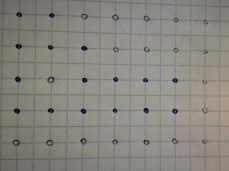
\includegraphics[width=0.33\textwidth, angle=90]{1b.jpeg}
	
	\aufgabe 2

\begin{align*}
\{l_2, l_3, l_5\} &\vDash p \vee q \\
\emptyset &\vDash AG(p \vee q) \\
\emptyset &\vDash EFAG(p \vee q)
\end{align*}

Da keine Location $AG(p\vee q)$ erfüllt, erfüllt auch keine $EFAG(p\vee q)$.

	 
\end{document}

